En ciencias de la computación, la técnica \textbf{Divide y Vencerás} es un paradigma de diseño
algorítmico que consiste en (i) dividir un problema en pequeñas partes que sean más manejables,
(ii) resolver cada subproblema individualmente y (iii) unificar las soluciones obtenidas 
para obtener el resultado final del algoritmo original \cite{Cormen2017}. 

El \textbf{objetivo} de esta práctica es resolver una serie de problemas algorítmicos aplicando
Divide y Vencerás, comparando la resolución que podemos considerar obvia respecto a la obtenida 
aplicando esta técnica. 

\subsection{Metodología}

Para realizar esta práctica se han implementado las soluciones a cada uno de los problemas
propuestos y se ha analizado su eficiencia respecto a los algoritmos ''obvios'' para resolverlos.
Con la finalidad de \textbf{automatizar} la ejecución y la generación de datos de eficiencia
de interés, hemos empleado el mismo programa que desarrollamos en \cite{Rojo2022}.
El funcionamiento interno del \textbf{Analizador} queda ilustrado en la figura 
\ref{fig:analizador} (más información en la referencia \cite{Rojo2022}). 

\begin{figure}[h]
    \centering
    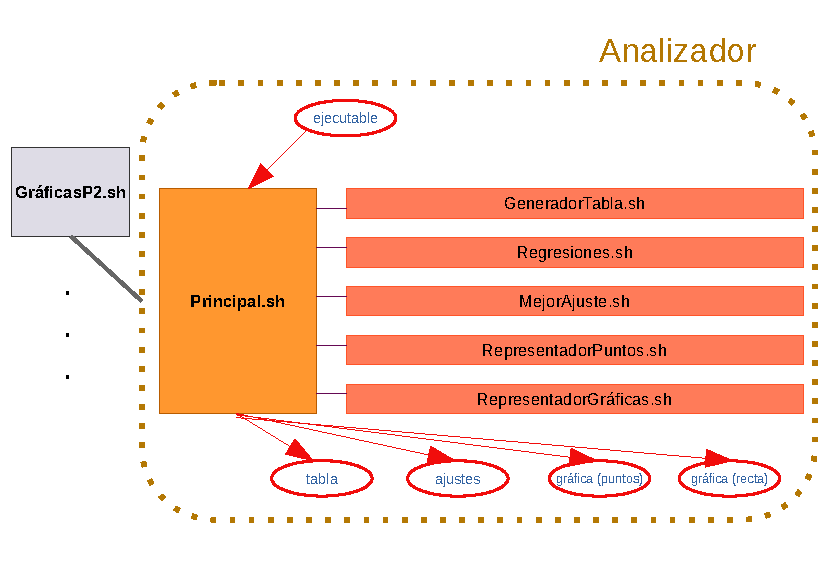
\includegraphics[scale=0.67]{img/esquema_graphkiller.pdf}
    \caption{Esquema de funcionamiento del \textbf{Analizador} \cite{Rojo2022}}
    \label{fig:analizador}
\end{figure}

\subsection{Equipo empleado}

Para el desarrollo de esta práctica, se ha empleado el equipo ?? con las siguientes características: % TODO